% Chapter 1 (from pres-main tex file)
% New Trends in Research
% Author: Javier Reyes

\subsection{Vivado HLx}

\begin{frame}
	\frametitle{Vivado HLx}
	Replacing ISE tools, the tool suite allows design, integration and implementation of systems for the Xilinx technologies.
	\vfill
	Included programs:
	\begin{itemize}
		\item Vivado HLx - High Level design
		\item Xilinx SDK - Software development 
		\item Vivado HLS - High Level Synthesis
		\item (Optional, external) Petalinux - Embedded Linux image building
	\end{itemize}
\end{frame}

\begin{frame}
	\frametitle{Vivado HLx}
	\begin{itemize}
		\item Interaction through GUI or native embedded TCL scripting language (commands either through the IDE console, or as file scripts). 
		\item Runs under Windows and Linux\footnote[frame]{Distro dependant, see \cite{UG973}} OS.
	\end{itemize}
\end{frame}

\begin{frame}
	\frametitle{IDiAL Server}
	Given the high requirements and the need to mantain a common work platform, a Virtual Machine is created in the IDiAL Server, where the tools are available to create/modify the designs.
	\vfill
	\begin{itemize}
		\item VM: U16x64D\_Vivado
		\item User: Javier
		\item Password: IDiAL
		\item OS: Ubuntu 16.04.3 Desktop
		\item IP-Address: 172.22.167.120
	\end{itemize}
\end{frame}

\begin{frame}[fragile]
	\frametitle{Basic install \& launch}
	\begin{lstlisting}[language=bash, basicstyle=\tiny\ttfamily, tabsize=2, commentstyle=\color{darkgray}, keywordstyle=\color{blue}, backgroundcolor=\color{lightgray}, morekeywords={chmod, sudo}, breaklines=true]
# Give executable permission to the installer file
chmod +x <installer_filename>.bin
# Executes the installer with root privileges
# Select the WebPack edition - no cost
# Include at least the SDK and the device Zynq in the content selection
# Select the installation folder
sudo ./<installer_filename>.bin
# After install, change to the driver cable installer folder
cd <vivado_folder>/data/xicom/cable_drivers/lin64/install_script/install_drivers/
# Execute the driver cable installer with root privileges
sudo ./install_drivers
# Create the apropiate environment for the suite to be launched
# Needs to be run everytime before launching Vivado
# Alternatively, can be added to the .bashrc to be executed automatically
source _vivado_installed_folder_/settings64.sh
# Launch the Vivado GUI, blocks the terminal when launched
vivado &
	\end{lstlisting}
	\begin{alertblock}{Constraint}
		{\small The Windows installer runs automatically the USB drivers, while in Linux it needs to be run after the Installation.}
	\end{alertblock}
\end{frame}

\begin{frame}
	\frametitle{Hardware Project}
	\begin{columns}
		\begin{column}{0.5\textwidth}
			\begin{figure}
				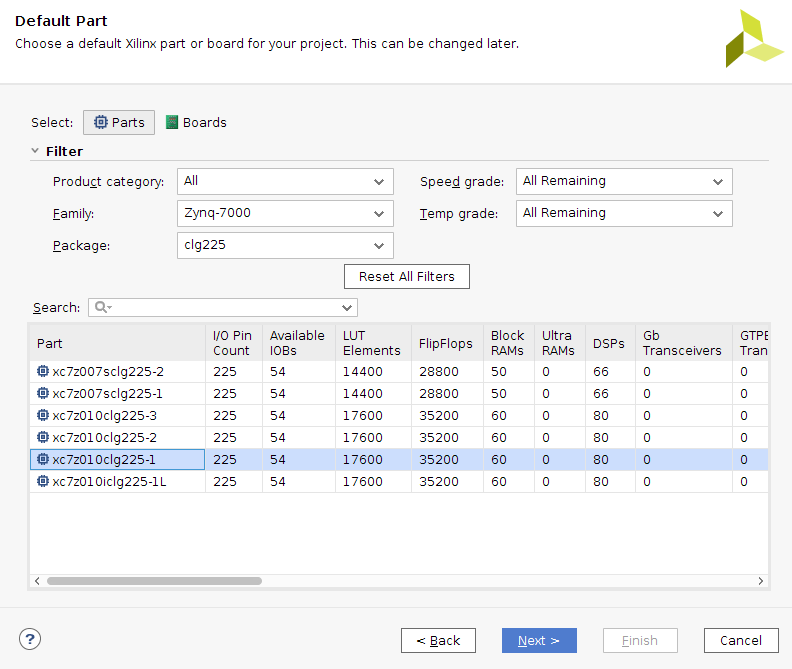
\includegraphics[width=\textwidth]{project-device.png}
				\caption{Vivado project - Device selection.}\label{fig:project-device}
			\end{figure}
		\end{column}
		\begin{column}{0.5\textwidth}
			\begin{itemize}
				\item Create a new project.
				\item Select RTL project type.
				\item Select the correspondent device.
				\item Create a new Block Design.
				\item Add the Zynq7 IP Core.
				\item Add/create any other necesary IP Core.
			\end{itemize}
		\end{column}
	\end{columns}
\end{frame}

\begin{frame}
	\frametitle{Hardware Project}
	\begin{columns}
		\begin{column}{0.4\textwidth}
			\begin{figure}
				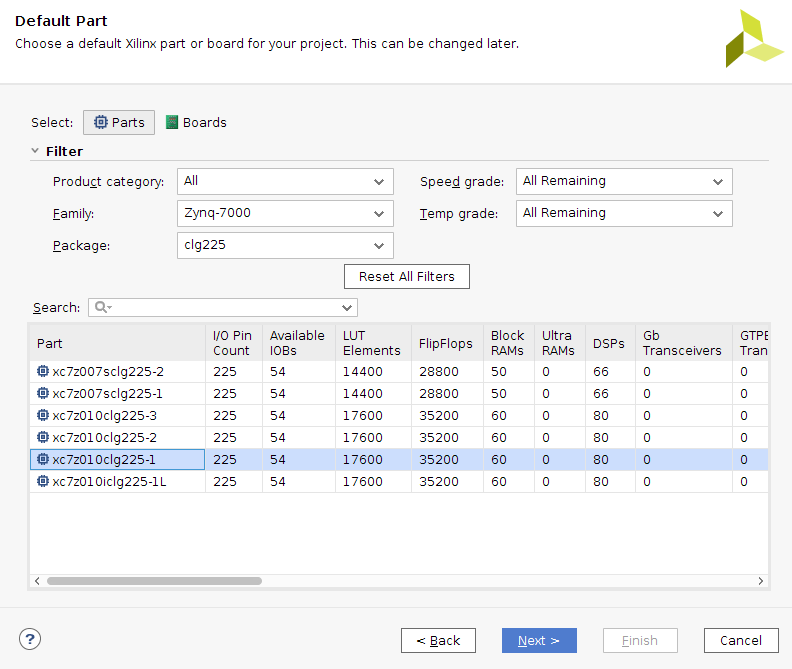
\includegraphics[width=\textwidth]{project-device.png}
				\caption{Vivado project - Device selection.}\label{fig:project-device}
			\end{figure}
		\end{column}
		\begin{column}{0.5\textwidth}
			\begin{itemize}
				\item Configure the IP Core.
				\begin{itemize}
					\item Apply the configuration in the TCL script, provided by the manufacturer.
					\item Ensure that all the required peripherals are enabled (CAN, USB, etc).
					\item Add/create any other necesary IP Core.
					\item Configure the IP Core.
				\end{itemize}
			\end{itemize}
		\end{column}
	\end{columns}
\end{frame}


% \lstinputlisting[language=tcl, basicstyle=\scriptsize\ttfamily, tabsize=2, commentstyle=\color{darkgray}, keywordstyle=\color{blue}, backgroundcolor=\color{lightgray}, morekeywords={create_project}, firstline=1, lastline=10, breaklines=true, numbers=left]{../../git/DAEbot/Devices/Zynqberry_OperatorPlus/zynqberryHW_CAN/create_project.tcl}

\subsection{Xilinx SDK}
